\subsection{Prediction Stencils and Coefficients}
\label{sec:background:stencils}

SZ3 and QoZ use several predefined prediction stencils and interpolation formulas. Fig.~\ref{fig:background:stencils} shows these stencils, and the equations below show how the interpolation formulas assign coefficients to their references.

\begin{figure}[htb]
\centering
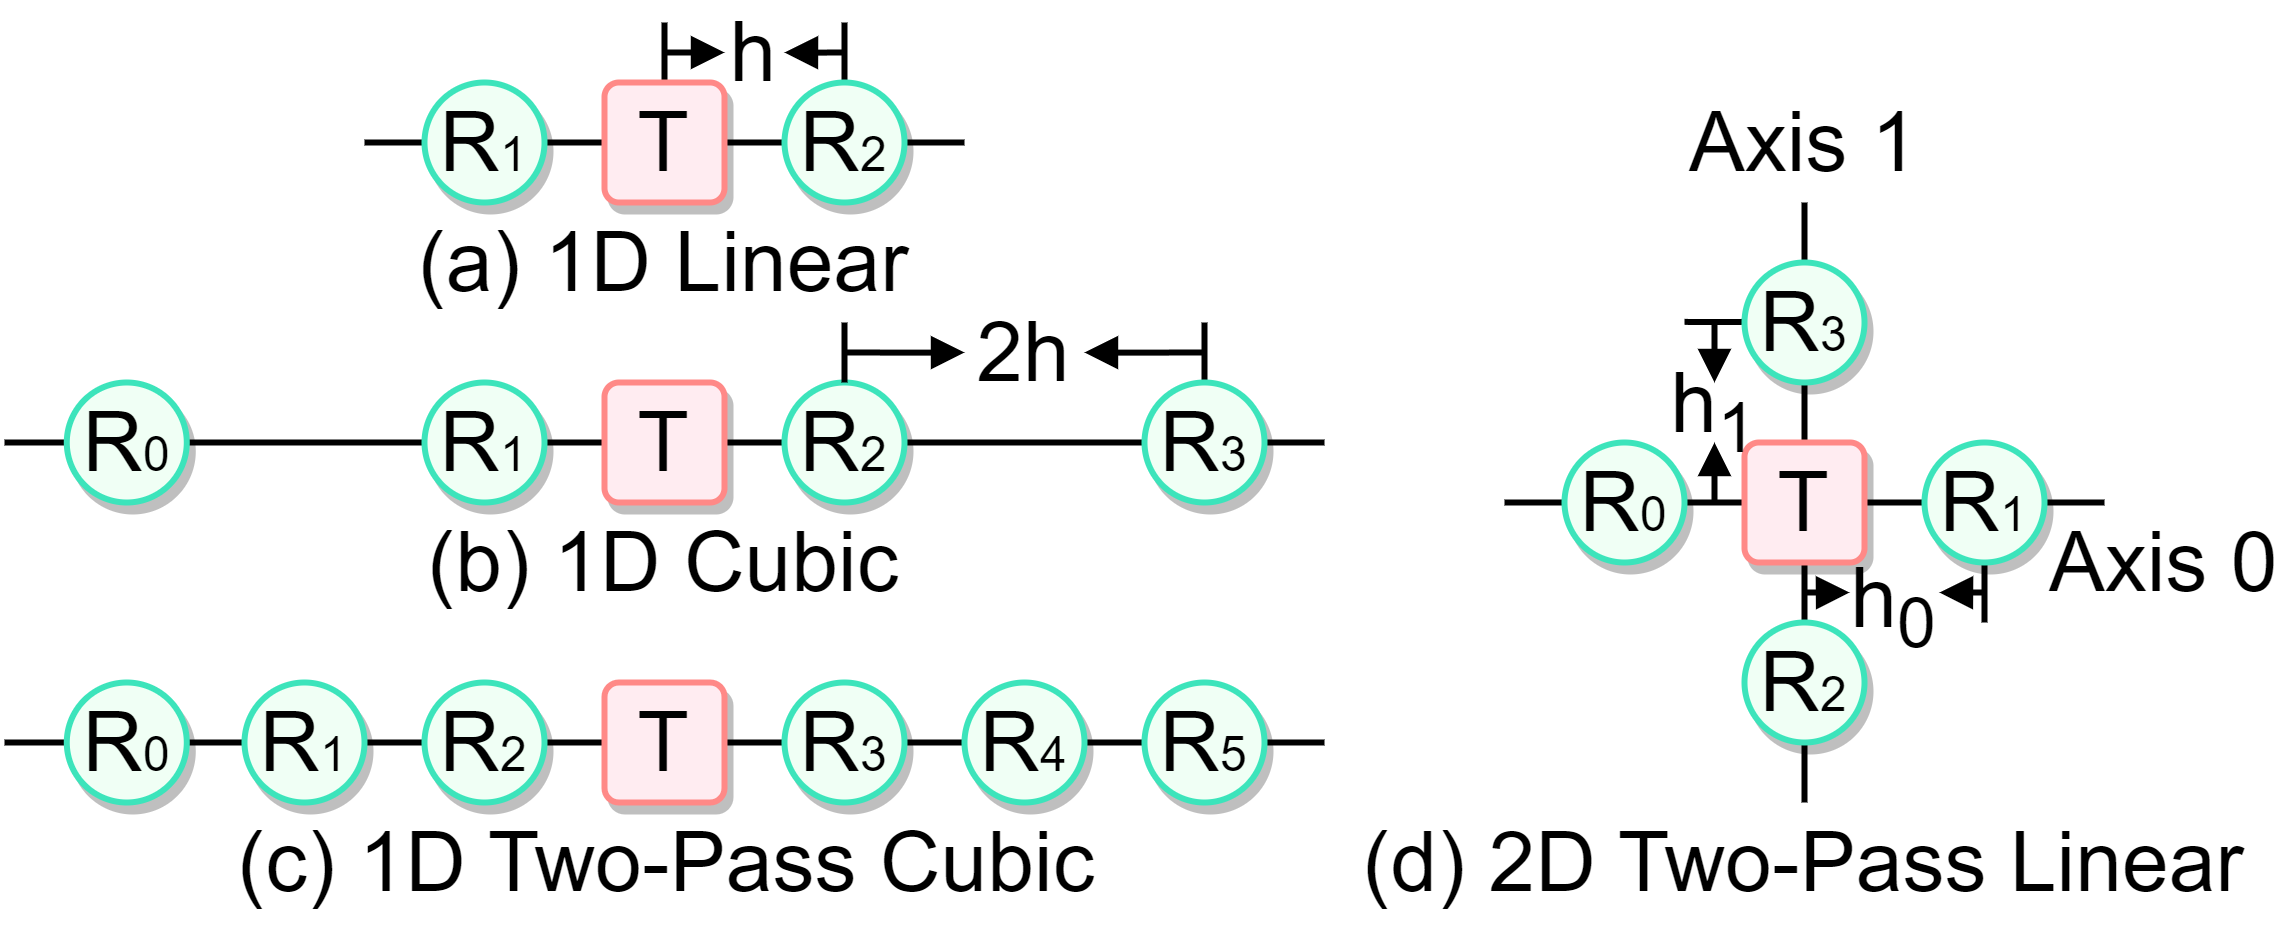
\includegraphics[width=0.8636\linewidth]{figs/3/prediction_stencils.png}
\caption{Prediction stencils in SZ3 and QoZ. $T$ is the value being predicted, and each $R_i$ is reconstructed before $T$ and available as its reference. ``Two-pass'' in stencils (c) and (d) means that a prediction round is divided into two passes. The illustrated stencils are used in the second pass, with some references reconstructed in earlier rounds and the others in the first pass of the current round. The reference spacing is $h$ in the one-dimensional stencils and $h_0$ or $h_1$ along each axis in (d).}
\label{fig:background:stencils}
\end{figure}

We first describe SZ3's two basic one-dimensional interpolation formulas. Linear interpolation uses the two-reference stencil in Fig.~\ref{fig:background:stencils}(a), while cubic interpolation uses the four-reference stencil in Fig.~\ref{fig:background:stencils}(b). With the prediction target at the origin and its nearest references at $-h$ and $h$, the two predictions are
\begin{align}
p_0^{\mathrm{lin}}&=\frac{1}{2}(\hat x_{-h}+\hat x_h),\label{eq:background:linear-interpolation}\\
p_0^{\mathrm{cub},1}&=\frac{9}{16}(\hat x_{-h}+\hat x_h)-\frac{1}{16}(\hat x_{-3h}+\hat x_{3h}).\label{eq:background:cubic-interpolation}
\end{align}

QoZ introduces the following alternative cubic-spline formula with the same four-reference stencil in Fig.~\ref{fig:background:stencils}(b):
\begin{equation}
\label{eq:background:qoz-cubic2}
p_0^{\mathrm{cub},2}=\frac{23}{40}(\hat x_{-h}+\hat x_h)-\frac{3}{40}(\hat x_{-3h}+\hat x_{3h}).
\end{equation}

QoZ also introduces a two-pass cubic interpolation scheme. It divides a prediction round into two dependent passes. In Fig.~\ref{fig:background:stencils}(c), $R_1$, $R_4$, and $T$ would ordinarily be targets in the same round. The first pass predicts and quantizes $R_1$ and $R_4$ with a four-reference cubic formula. The second pass predicts $T$ using their reconstructed values together with references reconstructed before the current round. QoZ provides two formulas for this second-pass layout:
\begin{align}
p_0^{\mathrm{6R},1}&=\frac{2}{3}(\hat x_{-h}+\hat x_h)-\frac{1}{6}(\hat x_{-2h}+\hat x_{2h}),\label{eq:background:qoz-six-reference-not-a-knot}\\
p_0^{\mathrm{6R},2}&=\frac{23}{31}(\hat x_{-h}+\hat x_h)-\frac{9}{31}(\hat x_{-2h}+\hat x_{2h})\nonumber\\
&\qquad+\frac{3}{62}(\hat x_{-3h}+\hat x_{3h}).\label{eq:background:qoz-six-reference-natural}
\end{align}

Equations~\eqref{eq:background:linear-interpolation} and~\eqref{eq:background:cubic-interpolation} assume that local data can be exactly represented by a linear or cubic function, respectively. Equations~\eqref{eq:background:qoz-cubic2}--\eqref{eq:background:qoz-six-reference-natural} are derived from cubic spline interpolation.

QoZ applies a similar two-pass organization to multidimensional interpolation. For the two-dimensional linear stencil in Fig.~\ref{fig:background:stencils}(d), two references are available before the round, and QoZ reconstructs the other two in the first pass. It then predicts $T$ in the second pass by combining linear predictions along the two axes. It assigns larger coefficients to axes with smaller sampled prediction errors. These coefficients are generated per block and stored as configuration metadata for decompression.

In all of the prediction formulas above, the coefficients sum to one, with equal coefficients assigned to references at symmetric positions along each interpolation axis.

\subsection{Configuration Granularity}
\label{sec:background:configuration-granularity}

SZ3 and QoZ jointly select prediction stencils and axis orders, but apply the resulting configurations at different granularities. When compressing three-dimensional data with one-dimensional interpolation, SZ3 selects one interpolation formula and one axis order for the whole file. The order is either $x,y,z$ or $z,y,x$. SZ3 repeats this three-round cycle throughout the coarse-to-fine prediction process.

QoZ typically selects a separate interpolation configuration, including the stencil and axis order, for each group of three rounds (an interpolation level in the QoZ paper). For each group, the QoZ implementation chooses between $x,y,z$ and $z,y,x$. With one frozen axis, along which QoZ never interpolates, QoZ instead selects a configuration for each two-round group and uses either order of the remaining axes. For example, freezing $z$ leaves $x,y$ and $y,x$ as the two choices.

Because every permitted axis order is a permutation of the active axes, both SZ3 and QoZ use each active prediction axis the same number of times within every configured cycle or group.
